%
% Beispielkapitel: Bedienung dieser Vorlage
%

% Zum Setzen von TeX-Quellcode, der nicht interpretiert werden soll
%\newcommand{\makro}[1]{\texttt{\textbackslash{}#1\{\}}}

\chapter{Additional topics}
\label{sec:advanced}

\section{Having a screen display}
\label{sec: advanced_screen}
When you are running around with your car, you cannot control it with the lab monitor. A laptop is recommended here  but you can also do it with other devices like smartphones (but it is difficult). A solution could be to connect the car to internet with Wifi and then access it from internet but you would be limited in range around the wifi box. What we will do is set up the car as an hotspot and connect directly to it with a device. Warning : if you use several cars during the course you will have to install this hotspot on each cars you are using.

\subsection{Create a wifi hotspot on the car}

First of all connect the wifi USB-key that goes with the car.

Click on the network icon and then go in the Edit connection section. Click on Add.

Choose Wifi and Next. You will be invited to enter a Wifi name and a SSID. Please be sure to put the name of your group in it (and especially do not choose simply "wifi-hotspot"). Then select the mode Infrastructure and the MAC Addres of the car.

Then go in the Security section, choose WPA\&WPA2 Personnal and give a password. Then in the IPv4 section make sure that the method "Shared with other computers" is selected. And save.

Then open a terminal and type the following command.

\shellcmd{gksu gedit /etc/NetworkManager/system-connections/wifi\_name}

And replace "Infrastructure" with "Ap"


This tutorial is explained on this page 
\hyperref[http://ubuntuhandbook.org/index.php/2014/09/3-ways-create-wifi-hotspot-ubuntu/]{http://ubuntuhandbook.org/index.php/2014/09/3-ways-create-wifi-hotspot-ubuntu/}



\subsection{Connect to the car}

You can connect to the car with the device of your choice by simply connecting to the wifi. There are different ways to control the car from now.

\subsubsection{Using SSH}


This is the most stable method and it has less errors with the car software. Make sure that the SSH service is correctly installed on the car.

For linux user, it is very easy. Simpy type on the guest laptop.

\shellcmd{ssh -X username\_on\_the\_car@local\_ip\_of\_the\_car} and connect with your username and password.

For Windows user, you can use install Linux on a virtual Machine and act like a Linux user but it could be very very slow. Or you could use the software PuTTY with Xming. You can find a tutorial on this website :

\hyperref[http://www.geo.mtu.edu/geoschem/docs/putty_install.html]{http://www.geo.mtu.edu/geoschem/docs/putty\_install.html}

Once again it can be very slow, so only use it to check for errors. To actually control the car, I would recommend using Teanviewer for any non Linux-users.


\subsubsection{Using Teamviewer}

The simpliest way to connect to the car using any devices or OS is Teamviewer. It works on Windows, Linux and Android/iOS devices. Of course a real computer is recommended obecause otherwise it could be very slow, unstable and not easy to use.

If Teamviewer is not installed on both host and guest machine, dowload and install it. Simply open the software on both machine. If a machine doesn't print out its IP address on the left side, go in Extra, Options, make sure that the LAN connections are enabled and restart.

\begin{figure}[htbp]
	\centering
		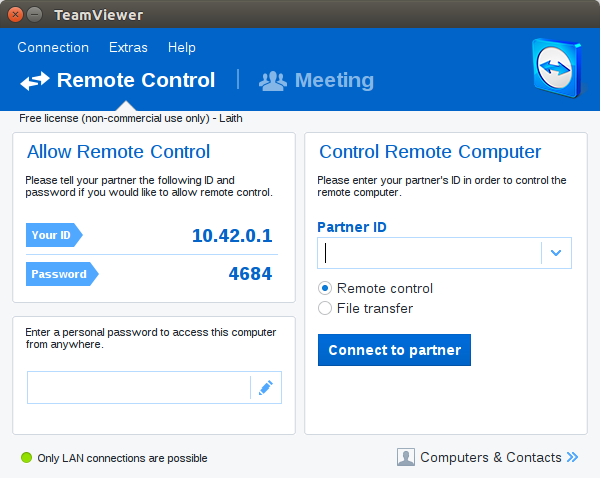
\includegraphics[width=\textwidth]{Teamviewer}
	\caption{Windows of Teamviewer}
	\label{fig:advanced_tv}
\end{figure}

Now on the guest machine, type the host' address and the password when it is asked. That's it !

Important note: for some reasons, Teamviewer has compatibility problems with RVIZ. RVIZ must be running before you even launch Teamviewer on the car.


\section{Recording and playing data, building your own map}
\label{sec:advanced_rosbag}

\subsection{Record a map}

To build a new map, you should obviously not have loaded the old one. That is why you only need to run the hardware and odom launch files (and not the move\_base one). The hardware file will allow to run all the devices of the car and the odometry one include the hector\_mapping node which we will use.

Once this nodes are running you can start recording the laser scanner data with a new terminal.

\shellcmd{rosbag record -O name\_of\_your\_bag /scan /tf} \\

If you look at this command line in details, it means you are recording all the data from the topics /scan (the laser scanner) and /tf (the transformation, see the section \refsec{tas_package_transformations}). The data will be saved in a .bag file. By default it is placed in your home directory.

Additionnally you can see the map building process in real time with Rviz (recommended to see if there is any errors). And now you can run around with the car to build your own map !

\subsection{Save your map and plug it in the TAS project}

The bag file you just created is literally a bag of data, it is not a map yet. You need to assemble this data into a map. In this tutorial you will see how to simulate this data while a ROS node (gmapping) is building it into a map using a SLAM algorithm. In order to do that close every processes you have launched and run roscore by simply typing it in a new terminal. That way you avoid any conflicting topics.

First you need to open a new terminal and reset the simulation time.

\shellcmd{rosparam set use\_sim\_time true}

Then run the gmapping node:

\shellcmd{rosrun gmapping slam\_gmapping scan:=scan}

Now simulate the data in a new terminal:

\shellcmd{rosbag play --clock name\_of\_your\_bag.bag}

Wait for the end of the process and record it:

\shellcmd{rosrun map\_server map\_saver}

You can also save the map with the name you want by using \shellcmd{rosrun map\_server map\_saver -f name\_of\_your\_map} instea of the previous command.


The tutorial is also explained at this address.

\hyperref[http://wiki.ros.org/slam_gmapping/Tutorials/MappingFromLoggedData]{http://wiki.ros.org/slam\_gmapping/Tutorials/MappingFromLoggedData}

Your map is now saved in your home directory with two files (.pgm and .yaml)

In order to use it in the TAS package, the two map files need to be in the folder catkins\_ws/src/tas\_group\_X/tas/launch/config/map\_server. Then the move\_base launch file should be modified so it could refer to the new map.

If you run run\_rviz.launch file (see the navigation section), you should see your new map.


\section{Version control with git}
\label{sec:advanced_git}

In order to get access to every data that are pre-installed and also to submit your project you need to use the Git software. It is also recommended to update your work regularly to prevent any problems on your hard-disk.

The all topic is covered on this website :
\hyperref[https://www.atlassian.com/git/tutorials/]{https://www.atlassian.com/git/tutorials/}
We will go through the main aspects of it.

\subsection{Import your working repository}

You already done it in the \refsec{tas_package_install} section. You can import (or clone) in the current folder with the command
\shellcmd{git clone <repo>}.

\subsection{Updating your local repository}

If the online git has been changed, you may want to update your local repository. You can dot it with the command \shellcmd{git pull} once you are in your local git repository.

\subsection{Updating your online repository}

Once you have made some changes on your hard disk, it could be a good idea to save this changes online.

First if all, go in your local git folder and check what changes have been made with
\shellcmd{git status}

Then you need to specify which files you want to update with the command "git add". If you want to update everything type:
\shellcmd{git add .}

You now need to commit your change. Use the command \shellcmd{git commit -m "message"} so every file that has been updated would have this message as a commit message.

And finally update the online repository with the command: \shellcmd{git push}

Don't forget to check on the online git if everything has been updated.


\section{Switching remote controller}
\label{sec:advanced_switch}

The car can be manually or automatically controlled whenever the hardware.launch file is running (or a launch file that includes it is running). It is not always said in the console but the first thing you need to do is connect the wiimote with the car even if you want a automatic control. You have to follow the line in section \refsec{tas_package_drivers} and be sure that the wiimote is controlling the wheels ! Then you can switch to automatic control (and vice versa) with the C-button of the wiimote.

\section{Recharging batteries}
\label{sec:advanced_recharge}

Since the car you are using are high power consuming, it may occur that the battery is empty. You will need to recharge it. Also don't forget to check the battery charging level with the button on its side before you need to use it.

If you need to charge it, turn on the power supply for the battery charging. Then press on the small black button "on/off" to turn on the Voltcraft box. Plug in the battery the same way as the picture \reffig{adv_charge} .

\begin{figure}[htbp]
	\centering
		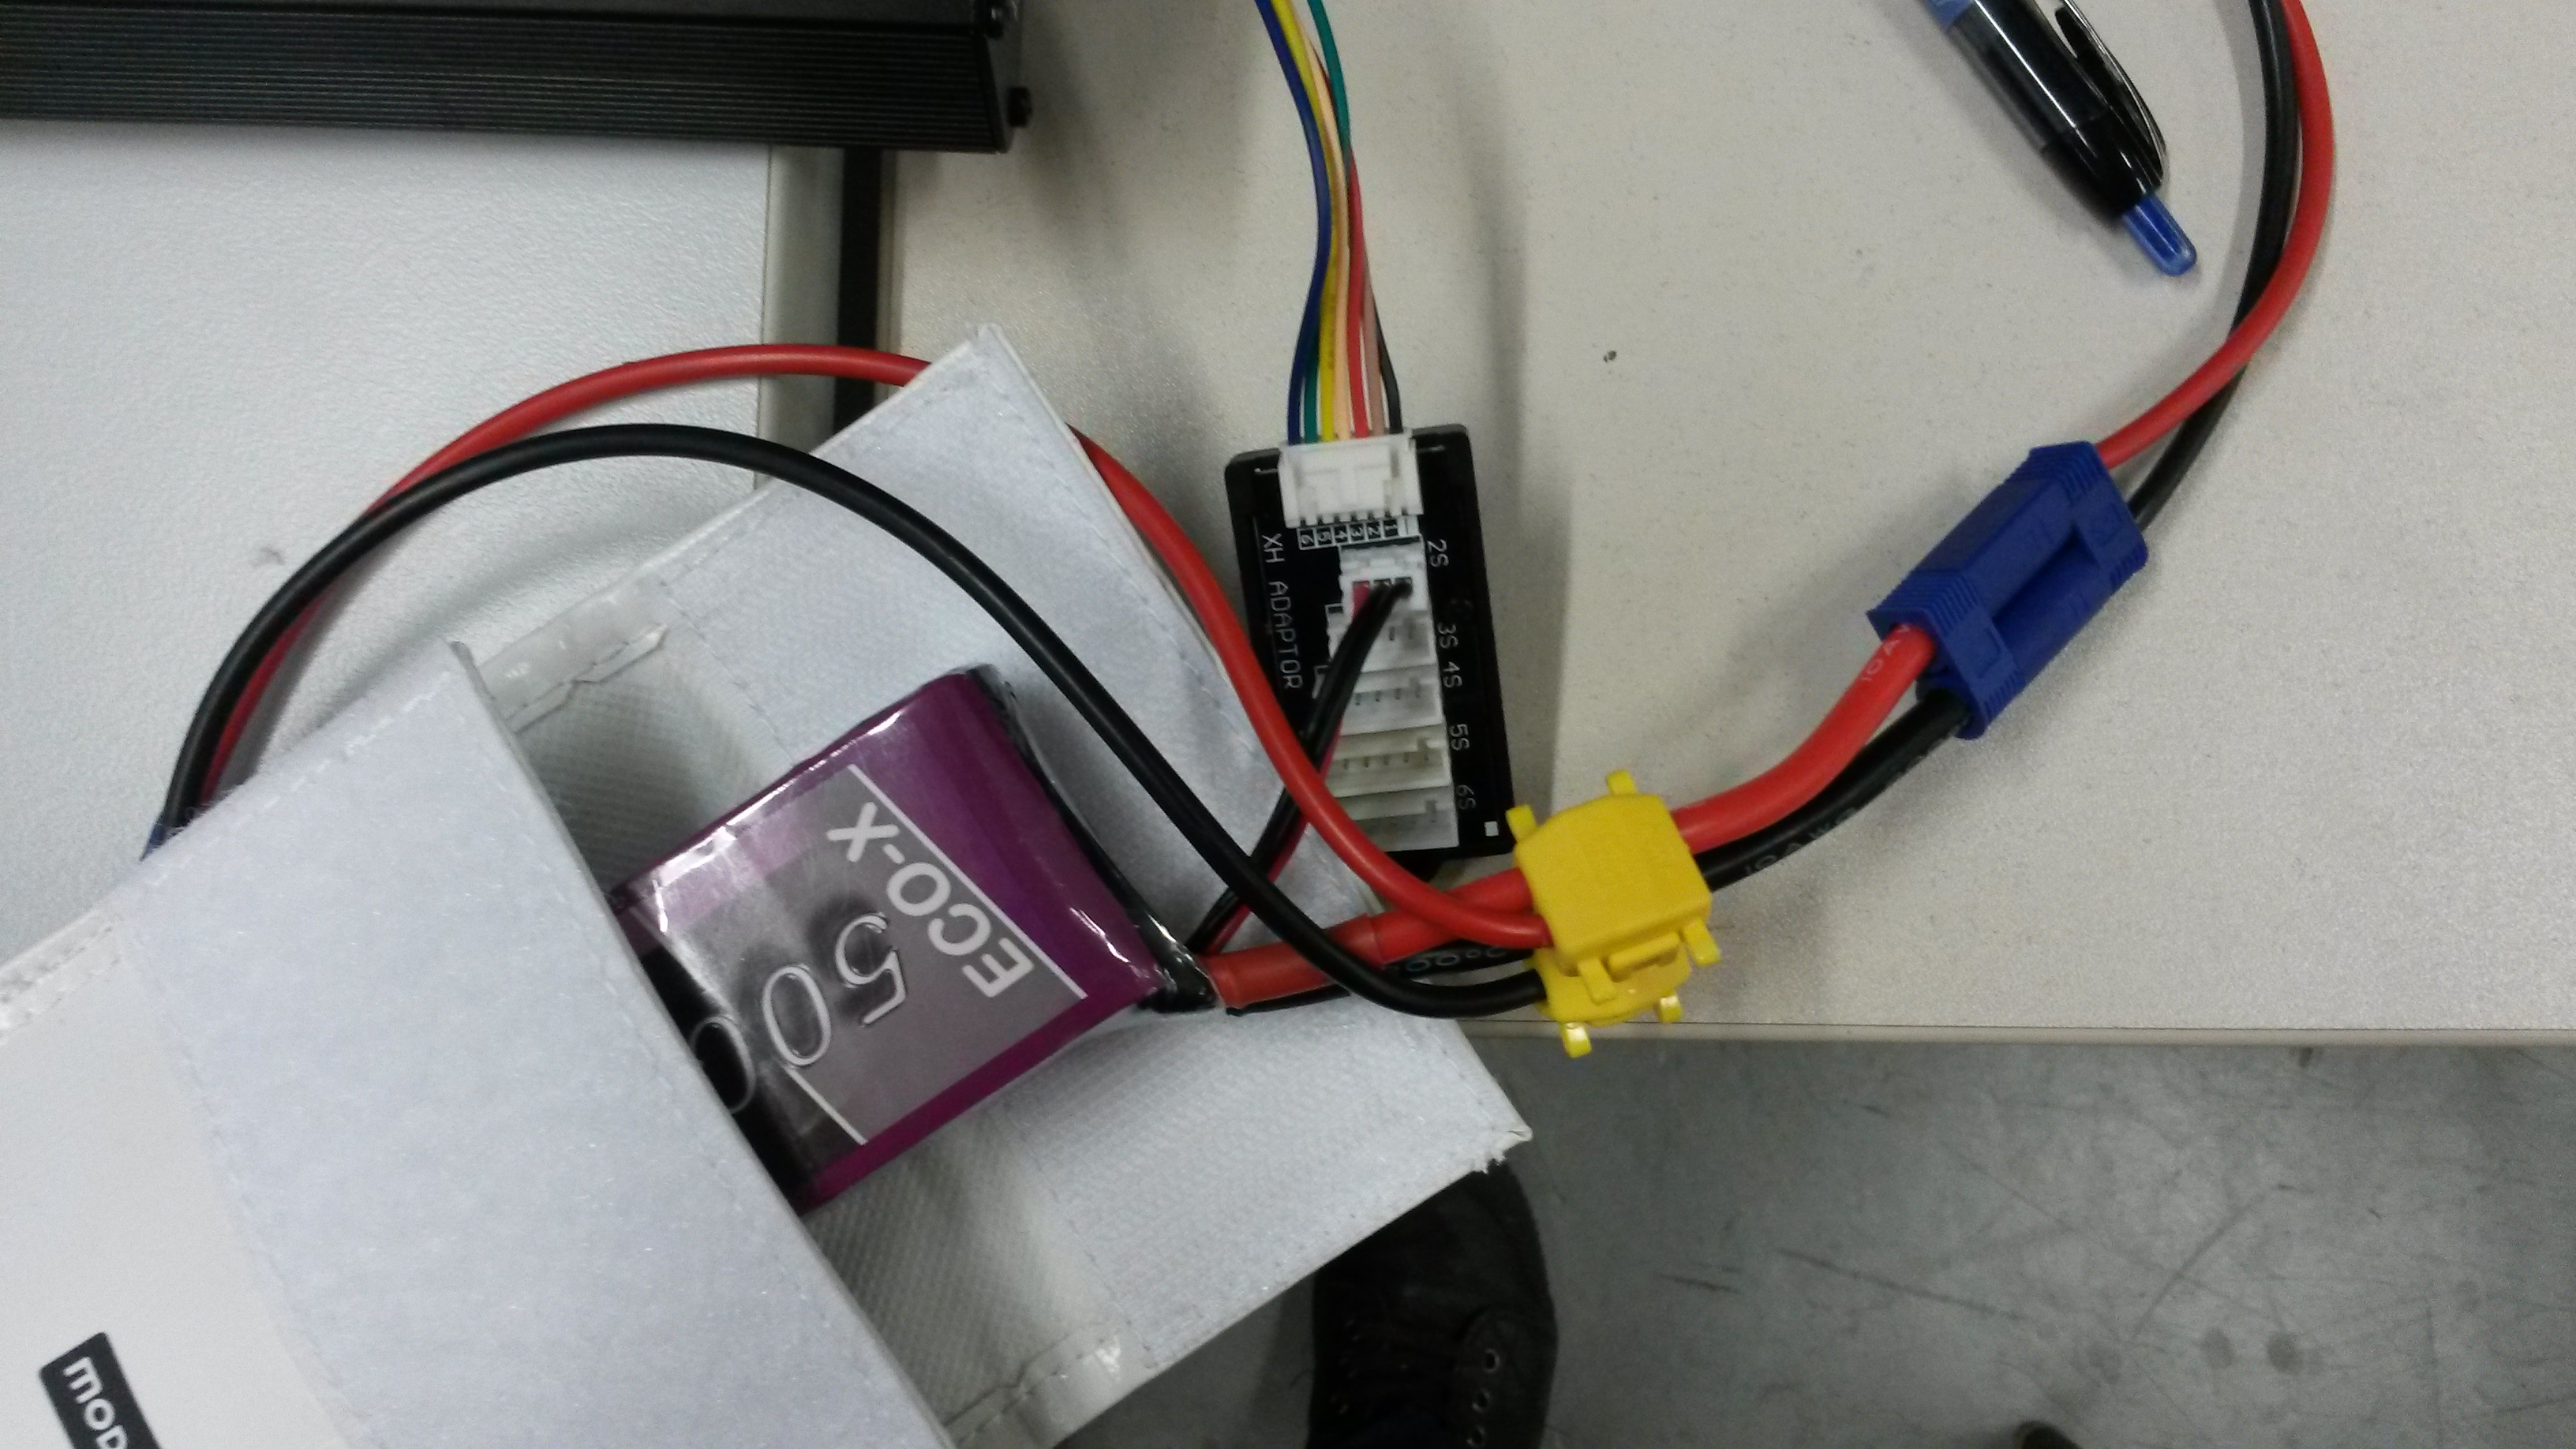
\includegraphics[width=\textwidth]{charge}
	\caption{Battery charging}
	\label{fig:adv_charge}
\end{figure}

Press on the Start-button until you heard several tones: the box will check the battery. When it is over (another beep) press once again the start button. The battery will charge and another burst of tones will tell you when it is over.

Important note : Always put the battery in its white case when charging and never let it charge when you are not in the N8 basement !



